\section{Valkuilen}
In theorie kan er van elke opstelling waarbij de punten niet allemaal colineair zijn een triangulatie worden gevonden, zie figuur \ref{colineair}. Echter door afronding bij de berekeningen zal er bij bijna colineaire punten geen juiste delaunay triangulatie gevonden worden, zie figuur \ref{almost_colineair}. 

\begin{figure}
	\center
	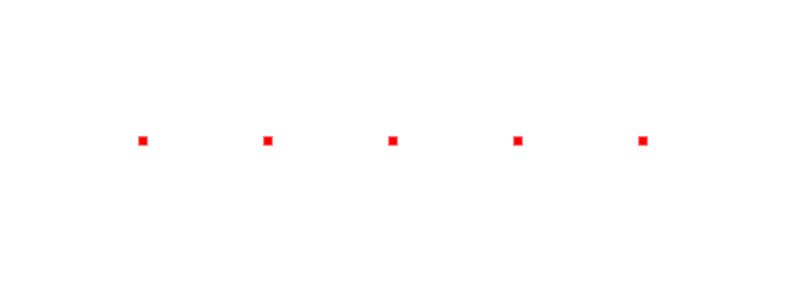
\includegraphics[width=0.4\textwidth]{colineair}
	\caption{Van colineaire punten kan geen triangulatie gevonden worden.}
	\label{colineair}
\end{figure}
\begin{figure}
	\center
	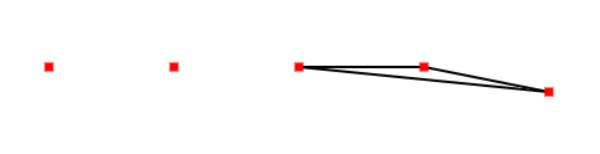
\includegraphics[width=0.4\textwidth]{almost_colinair}
	\caption{Van bijna colineaire punten kan geen triangulatie gevonden worden door afrondingsfouten bij berekeningen.}
	\label{almost_colineair}
\end{figure}
